\documentclass[xcolor=dvipsnames]{beamer}
\usetheme{CambridgeUS}
\usepackage[labelformat=simple,
labelsep=period,
font={footnotesize},     %scriptsize, footnotesize, small, normalsize
labelfont=bf,
width=0.9\textwidth,
justification=justified,
singlelinecheck=false
]{caption}
\usepackage[utf8]{inputenc}
\usepackage[spanish, es-tabla]{babel}
\usepackage{amsmath}
\usepackage{subfigure}
\usepackage{amsfonts}
\usepackage{amssymb}
\usepackage{qtree}
\usepackage{tikz}
\usetikzlibrary{calc}
\usepackage{pgfplots,pgfplotstable}
\usepgfplotslibrary{statistics}
\usepackage[T1]{fontenc}
\usepackage{bera}
\usepackage{pstricks-add}
\usepackage[capposition=top]{floatrow}
\usepackage{graphicx}
 \usepackage{ragged2e}
 \usepackage{float}
 \usepackage[labelformat=simple,
 labelsep=period,
 font={footnotesize},     %scriptsize, footnotesize, small, normalsize
 labelfont=bf,
 width=0.9\textwidth,
 justification=justified,
 singlelinecheck=false
 ]{caption}
 \usepackage[justification=centering]{caption}
\setbeamersize{text margin left=5pt,text margin right=25pt}
\captionsetup[figure]{labelfont={color=Brown}}
\captionsetup[table]{labelfont={color=Brown}}
\tikzset{
	% Two node styles for game trees: solid and hollow
	solid node/.style={circle,draw,inner sep=1.5,fill=black},
	hollow node/.style={circle,draw,inner sep=1.5}
}
%%%%%%%%%%%%%%%%%%%%%%%%%%%%%%%%%%%%%%%%%%%%%%%%%%%%%%%%
%%% PAra el diagrama de la diapostiva 10
\usepackage{smartdiagram}
\usetikzlibrary{shapes.geometric} % required in the preamble
\smartdiagramset{
	module minimum width=3cm,
	module minimum height=1cm,
	text width=4.5cm,
	circular distance=3cm,
}
%%%%%%%%%%%%%%%%%%%%%%%%%%%%%%%%%%%%%%%%%%%%%%%%%%%%%%%%%%%
\def\angle{0}
\def\radius{2}
\def\cyclelist{{"orange","blue","red","green"}}
\newcount\cyclecount \cyclecount=-1
\newcount\ind \ind=-1	


	
\author[Carlos Cardona]{Carlos Cardona}
\title{Análisis Cuantitativo I}
\subtitle{Diseño, Medición y Medidas de Tendencia Central}
\institute[URosario]{Universidad del Rosario}
\date{3 de febrero de 2017}
\begin{document}
\maketitle

%%%%%%%%%%%%%%%%%%%%%%%%%%%
\begin{frame}{Quiz}
	\justifying
	Indique si la siguiente afirmación es verdadera o falsa. Si es falsa justifique su respuesta.
	\begin{itemize}
		\justifying
		\item {\bf Tema A:} El diferencial de salarios entre nativos e inmigrantes es un constructo de la definición operacional \emph{prejuicio}.
		\item {\bf Tema B:} La estadística descriptiva busca alcanzar un estadístico a partir de un parámetro.
	\end{itemize}
\end{frame}

\section{Repaso}
\begin{frame}{Repaso}
\begin{itemize}
\item El número diario promedio de mensajes de texto que envían los colombianos es un parámetro o un estadístico?
\item Si cada uno elige su programa favorito, esta variable seria nominal, ordinal o de razón?
\item La edad es una variable discreta o continua?
\item A la hora de graficar una variable de escala ordinal, cuál(es) de los tipos de gráfica vistos en la clase anterior sería(n) viables?
\end{itemize}
\end{frame}

%%%%%%%%%%%%%%%%%%%%%%%%%%%%%%%
\section{Diseños de Investigación}

\begin{frame}{Diseño de Investigación}
\begin{itemize}
\justifying
\item La mayoría de fenómenos que estudian las ciencias sociales tienen múltiples causas.
\item  Las teorías, en cambio, se enfocan en una de las causas e ignoran las demás.
\item La naturaleza multivariada de los conceptos puede llevar a conclusiones engañosas.
\item Por ejemplo, algunos estudios han mostrado que la raza (X) en EE.UU está relacionada con la participación política (Y). Donde los anglosajones participan más que las demás razas.
\end{itemize}
\end{frame}


\begin{frame}
	\begin{itemize}
		\justifying
\item La conclusión podría ser errónea si se lleva a cabo una comparación más compleja. Personas de diferentes razas (X) tienen condiciones socioeconómicas diferentes (Z), las cuales se asocian tanto con la raza y también afectan la participación política.
\item Las \emph{comparaciones} están en la esencia de la ciencia. Si evaluamos una teoría que relaciona X y Y, la labor científica es hacer todo lo posible para asegurarse que no existen otras influencias (Z) que interfieran con las comparaciones realizadas.
\item La variable X se conoce como la \emph{variable independiente}, aquella que es denotada como causa. Por otro lado, la variable Y es la \emph{dependiente}.

	\end{itemize}
\end{frame}

\begin{frame}
	\begin{itemize}
		\justifying
\item Existen diferentes estrategias, o diseños investigativos, que pueden usar para encontrar conclusiones, creíbles y no influenciadas por factores externos, de ciertas teorías.
\item Las dos técnicas más usadas y efectivas son:
\begin{enumerate}
\item Los experimentos.
\item Los estudios observacionales. 
\end{enumerate}
	\end{itemize}
\end{frame}

\begin{frame}{El Diseño Experimental}
\begin{itemize}
\justifying
\item Supongan que son un candidato a un cargo político. Además, tienen aún presupuesto para usarlo en publicidad que contraste sus habilidades con las del oponente. 
\item La pregunta sería: ¿La publicidad funcionará con los votantes?\footnote{Wattenberg, Martin P. \& Craig Leonard Brians. 1999. “Negative Campaign Advertising: Demobilizer or Mobilizer?” American Political Science Review.}
\item La aproximación estándar para una situación como esta es conducir un \emph{experimento}.
\end{itemize}
\end{frame}

\begin{frame}{El Diseño Experimental}
	\begin{block}{Definición}
		\centering
Un experimento es un diseño investigativo en el cual, el investigador controla y asigna aleatoriamente valores de la variable independiente a los participantes.
	\end{block}
	\begin{itemize}
		\justifying
		\item Los participantes del experimento serán divididos de manera \emph{aleatoria} a un {\bf grupo tratamiento} y a un {\bf grupo control}.
		\item ¿Por qué es importante la asignación aleatoria?
\pause		\item La asignación aleatoria descontamina la comparación entre ambos grupos de otras influencias.
	\end{itemize}
\end{frame}

\begin{frame}{Caracterízticas e Inconvenientes de un Diseño Experimental}
\begin{itemize}
\justifying
\item Validez Interna-¿Qué tan confiables son las conclusiones?
\item Tipos de Experimentos:
\begin{enumerate}
\item Encuesta Experimental.
\item Experimento de Campo.
\item Experimentos Naturales.
	
\end{enumerate}
\item Desventajas:
\begin{enumerate}
\item No toda variable independiente es manipulable. 
\item Bajos niveles de validez externa- Muestreo por conveniencia y el estímulo.
\item Aspectos éticos.
\item X es la principal causa?
\end{enumerate}
\end{itemize}
\end{frame}

\begin{frame}{Estudios Observacionales}
\begin{itemize}
\justifying
\item La implementación de un experimento a menudo resulta ser inviable, y otras veces imposible.
\item Como resultado de esto, la experimentación no es el diseño más común entre las ciencias sociales.
\item En casos donde no se puede controlar la exposición a la variable de interés, la única elección es observar al mundo como si ya existiera y hacer las comparaciones entre \emph{individuos} o entre cantidades agregadas que varían en el tiempo.

\item Los estudios observacionales no son experimentos, pero tratan de emularlos.
\end{itemize}
\end{frame}

\begin{frame}{Estudios Observacionales}
\begin{block}{Definición}
Un estudio observacional es un diseño donde el investigador no tiene control sobre los valores de la variable independiente, la cual ocurre naturalmente.
\end{block}
\begin{itemize}
\justifying
\item Sin embargo, es importante que exista variabilidad tanto en la variable dependiente como la independiente.
\item Debido a la incapacidad de manipular la variable independiente, algunos académicos los denominan estudios correlacionales.
\item Tipos de estudios observacionaes:
\begin{enumerate}
\item Corte Transversal
\item Corte Longitudinal
\item Series de Tiempo
\end{enumerate}
\end{itemize}
\end{frame}

%%%%%%%%%%%%%%%%%%% La medición
\section{El problema de la Medición}
\begin{frame}{La medición}
	\begin{itemize}
\justifying
\item La medición es un ``problema'' para todas las ciencias.
\item Para las ciencias físicas, el problema de la medición se reduce a la instrumentación, bajo el cual los científicos desarrollan protocolos para medir ciertos fenómenos.
\item Las ciencias sociales, por el contrario, rara vez tienen concenso sobre cómo medir sus conceptos importantes.
\item Más importante es que las ciencias sociales lidian con un objeto díficil de predecir: el ser humano. 
\end{itemize}
\end{frame}

\begin{frame}
\begin{itemize}
\justifying
\item Es un error pensar que para todas las disciplinas de las ciencias sociales, la medición es igual de problemática.
\item Consideremos el objeto de estudio en la mayoría de investigaciones de economía: el dólar, el euro o el peso.
\item Si el concepto de interés es el ``producto económico'', resulta bastante sencillo obtener una observación empírica que sea consistente $ \rightarrow $ el PIB.
\item Luego de tener clara esta medida, los economistas pueden ir al siguiente (y más interesante) paso en el proceso científico: preguntarse qué causa 	mayor o menor crecimiento en el producto. \end{itemize}
\end{frame}

\begin{frame}
\begin{itemize}
\justifying
\item No todo concepto en economía es medido con tal facilidad.
\item ¿Por qué algunos son pobres mientras que otros no?
\item Aunque todos sabemos que la pobreza existe, medirla es complicado. 
\item Los economistas rara vez (pero ocasionalmente) tienen obstáculos con la medición. El extremo opuesto del espectro sería la psicología.
\end{itemize}
\end{frame}

\begin{frame}
	\begin{itemize}
\justifying
\item El comportamiento humano, el proceso cognitivo y las emociones son conceptos extremamente complicados de medir.
\item La depresión y la ansiedad existen pero ¿cómo medirlas?
\item Es relevante tener una medición precisa de ellas para poder evaluar si la terapia clínica o los antidepresivos son efectivos.
\item La sociología y la ciencia política se localizan entre los extremos que son la economía y la psicología.
\item Los siguientes conceptos críticos son ejemplos que tienen complicaciones a la hora de ser cuantificados:
\begin{enumerate}
\item Democracia.
\item Capital Social.
\item Prejuicio.
\end{enumerate}
\end{itemize}

\end{frame}

%%%%%%%%%%%%%%%%%%%%%%%%%%%%%%%%%%%%%%%%%%%%%
\section{Problemas al medir conceptos de interés}
\begin{frame}{Claridad Conceptual}
	\begin{itemize}
		\justifying
		\item El primer paso para medir cualquier fenómeno es tener un sentido claro del concepto de interés.
		\item En muchos casos, es un trabajo difícil y revelador.
		\item Aún en ejemplos que parecen sencillos, el tener claro lo que queremos decir con los conceptos es más complejo de lo que parece.
\item La \emph{mejor} medida de un concepto depende de cuáles son nuestros objetivos teóricos.
	\end{itemize}
\end{frame}

\begin{frame}{Confiabilidad}
\begin{itemize}
\justifying
\item Una definición operacional es confiable si es repetible y consistente.
\item Si al aplicar la misma regla de medida a una observación produce los mismos resultados, la medida es consistente.
\item Confiabilidad vs. Variabilidad.
\item Es sumamente importante al momento de codificar eventos o textos para una análisis cuantitativo.
\end{itemize}
\end{frame}

\begin{frame}{Sesgo de Medida y Confiabilidad}
\begin{itemize}
	\justifying
\item Una preocupación que surge con cualquier técnica de medición es el sesgo de medida.
\item El sesgo de medida es el sobre-reporte o sub-reporte sistemático de los valores de una variable.
 \item Imaginemos que estamos frente a la elección de dos definiciones operacionales de una misma variable. 
\item La definición operacional A es confiable y sesgada, y la definición B es insesgada y no confiable. ¿Cuál sería la definición a usar?
\end{itemize}
\end{frame}

\begin{frame}
	\begin{itemize}
		\justifying
 \item Aunque el sesgo de medida es un problema para alguien que quiere saber los ``verdaderos'' valores de una variable, no es un gran inconveniente a la hora de evaluar teorías.
 \item Al indagar teorías, estamos buscando patrones generales entre dos variables.
 \item ¿Con valores más altos de X, tendemos a ver valores mas altos de Y? O valores más bajos?
 \item Si la medida de X está sesgada hacia arriba, el mismo patrón será visible en la asociación con Y.
 \item Si X no es confiable, la relación entre Y y X no será clara. 
\end{itemize}
\end{frame}

\begin{frame}{Validez}
\begin{itemize}
\justifying
\item La validez es la característica más importante de una medida.
\item Esta se refiere a cuan adecuadamente una medida refleja el concepto en consideración.
\item No existe una fórmula  simple que la validez de una medida en una escala de 0 a 100. 
\item En cambio, nos basamos en la superposición de varios criterios:
\begin{enumerate}
\item Validez Aparente.
\item Validez Predictiva.
\item Validez de Constructo.
\item Validez de Contenido.
\end{enumerate}
\end{itemize}
\end{frame}

\begin{frame}{Confiabilidad vs. Validez}
\begin{itemize}
\item Claramente, queremos medidas que sean tanto confiables como válidas.
\item Sin embargo, existe una disyuntiva entre ambas características.
\item Entre mayor variación le permitamos tener a un concepto, es más probable crear desacuerdos en relación a si este aplica a una situación particular.
\item En cierta medida, este dilema explica la persistencia de dos enfoques diferente de investigación social: el cualitativo y el cuantitativo.
\item En la generalización más simple, los métodos cualitativos tienden a ser más validos y los cuantitativos más confiables. 
\end{itemize}
\end{frame}

\begin{frame}{Controversia: Midiendo la Democracia}
\begin{itemize}
\justifying
\item Se podría estar tentado a evaluar la democracia como una condición absoluta, pero podríamos obviar el hecho de que hay países más democráticos que otros.
\item Por lo tanto, se podría pensar la democracia como un \emph{continuum}\footnote{Elkins, Zachary. 2000. “Gradations of Democracy? Empirical Tests of Alternative
	Conceptualizations.” American Journal of Political Science}.
\item Definir un continuo de valores entre democracia y totalitarismo no es sencillo.
\item ¿ A qué nos referimos con democracia? ¿Cuáles son los elementos básicos que conforman un gobierno más o menos democrático?
\end{itemize}
\end{frame}

\begin{frame}{Polity IV}
	\begin{itemize}
\justifying
\item La medida más conocido -no necesariamente más aceptada- es la del proyecto Polity IV.
\item Miden la democracia anualmente mediante valores que oscilan de -10 (fuertemente autocrático) a 10 (fuertemente democrático) para cada país de 1800 a 2012.
\item Esta definición operacional tiene cuatro componentes:
\begin{enumerate}
\item Regulación en la elección del ejecutivo.
\item Competencia en la elección del ejecutivo.
\item Que tan abierta es la elección del ejecutivo.
\item Restricciones al ejecutivo.
\end{enumerate}
	\end{itemize}

\end{frame}

\begin{frame}
\begin{itemize}
\justifying
\item Para cada una de esas dimensiones, expertos valoran cada país en una escala.
\item Por ejemplo, para el primer criterio utilizan los siguiente valores: \begin{itemize}
\item +3 = competición regular entre grupos reconocidos
\item +2 = competencia transicional.
\item +1 = patrones restringidos de competencia o de facciones.
\item 0 = no hay competencia.
\end{itemize}
\end{itemize}
\end{frame}

\begin{frame}{Polity IV: Colombia}
\begin{figure}[H]
	\centering  
	\caption{ } 
	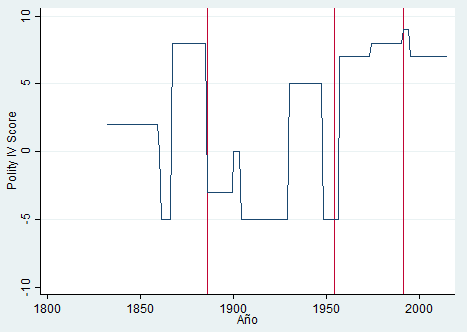
\includegraphics[width = 0.6\textwidth]{./cap1}
\end{figure}
\end{frame}

\begin{frame}{Polity IV: Estados Unidos}
	\begin{figure}[H]
		\centering  
		\caption{ } 
		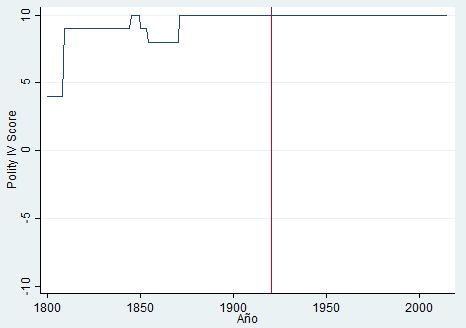
\includegraphics[width = 0.6\textwidth]{./cap2}
	\end{figure}
\end{frame}

%%%%%%%%%%%%%%%%%%%%%%%% Distribución $$$$$$$$$$$$$$$$$$$$$$$$$$$
\section{Distribución de Frecuencia}

\begin{frame}{Distribución de Frecuencia}
	\begin{itemize}
		\justifying
		\item Retomemos el concepto de distribución de frecuencia de la clase pasada... 
		\pause \item El histograma es una herramienta útil para presentar la distribución de una variable de razón.
		\item Por ejemplo: la distribución del número de hijos de un país. 
	\end{itemize}
	\begin{center}
		
		\scalebox{0.5}{
			\begin{tikzpicture}
			\begin{axis}[
			ybar,
			ymin=0,
			ylabel={Número de Habitantes (en millones)},
			xlabel={Número de Hijos },
			]
			\addplot +[
			hist={
				bins=7,
				data min=0.5,
				data max=4
			}   
			] table [y index=0] {data.csv};
			\end{axis}
			\end{tikzpicture}}
	\end{center}
	
\end{frame}

\begin{frame}{Curva de Distribución de Frecuencia}
	\begin{itemize}
		\justifying
		\item Cuando una población consiste en valores numéricos de una escala de razón, se acostumbra a dibujar la distribución con una curva suavizada. 
		
	\end{itemize}
	\begin{center}
		\scalebox{0.6}{\begin{tikzpicture}
			\begin{axis}[axis lines=left, ticks=none,xmin=0,ymax=0.5,ylabel={Número de Habitantes (en millones)},
			xlabel={Número de Hijos },]
			\addplot[thick,black, no markers, samples=200, domain=0:5] {abs(x)*exp(-x)};
			
			\end{axis}
			\end{tikzpicture}}
	\end{center}
\end{frame}

\begin{frame}
	\begin{itemize}
		\justifying
		\item Muchos textos definen la curva de distribución de frecuencias como un sustituto del histograma o del polígono.
		\item La sustitución es apropiada porque la curva suavizada se presenta más como una estimación de la distribución de los valores en la población. 
		\item La distribución poblacional más común es \emph{la curva normal}. 
		\item La distribución normal es \emph{simétrica}, es decir, equilibrada a ambos lados.
	\end{itemize}
\end{frame}

\begin{frame}{La distribución normal}
	\begin{center}
		\scalebox{0.8}{
			\begin{tikzpicture}
			\begin{axis}[axis lines=left, ticks=none,xmax=3, xmin=-3,ymax=1.5, xlabel={X},]
			\addplot[thick,black, no markers,samples=200] {exp(-x^2)};
			\end{axis}
			\end{tikzpicture}}
	\end{center}
	\begin{itemize}
		\justifying
		\item A partir de acá, siempre que aparezca el término \emph{distribución}, imaginen una gráfica de distribución de frecuencia. 
	\end{itemize}
\end{frame}

\begin{frame}{La Forma de una Distribución de Frecuencia}
	\begin{itemize}
		\justifying
		\item En vez de presentar la figura de la distribución de frecuencia, se puede describir al enumerar sus características.
		\item Existen tres características que describen completamente una distribución:
		\begin{enumerate}
			\item Forma.
			\item Tendencia Central.
			\item Variabilidad.
		\end{enumerate}
		\item La forma de una distribución puede ser clasificada en \emph{simétrica} o \emph{sesgada}. \end{itemize}
\end{frame}

\begin{frame}{La Forma de una Distribución de Frecuencia}
	{\sc Distribución Sesgada Negativamente}
	\begin{center}
		\scalebox{0.8}{
			\begin{tikzpicture}
			\begin{axis}[axis lines=left, ticks=none,xmax=0.5,ymax=0.5, xlabel={X}]
			\addplot[thick,black, no markers, samples=200, domain=-5:0] {-x*exp(x)};
			
			\end{axis}
			\end{tikzpicture}}
	\end{center}
\end{frame}

\begin{frame}{La Forma de una Distribución de Frecuencia}
	{\sc Distribución Simétrica}
	\begin{center}
		\scalebox{0.8}{
			
			\begin{tikzpicture}
			\begin{axis}[axis lines=left, ticks=none,xmax=3, xmin=-3,ymax=1.5, xlabel={X}]
			\addplot[thick,black, no markers,samples=200] {1.5*exp(-x^2)};
			\end{axis}
			\end{tikzpicture}
		}
	\end{center}
\end{frame}

\begin{frame}{La Forma de una Distribución de Frecuencia}
	{\sc Distribución Sesgada Positivamente}
	\begin{center}
		\scalebox{0.8}{
			
			\begin{tikzpicture}
			\begin{axis}[axis lines=left, ticks=none,xmin=0,ymax=0.5, xlabel={X}]
			\addplot[thick,black, no markers, samples=200, domain=0:5] {abs(x)*exp(-x)};
			
			\end{axis}
			\end{tikzpicture}
		}
	\end{center}
\end{frame}

%%%%%%%%%%%%%%%%%%%%%%% Medidas de Tendencia Central%%%%%%%%%
\section{Medidas de Tendencia Central}
\begin{frame}{Tendencia Central}
	\begin{itemize}
		\justifying 
		\item El propósito principal de la estadística descriptiva es organizar y resumir un conjunto de valores.
		\item El método más común de hacer esto es encontrar un valor \emph{puntual} que defina el valor promedio y sea representativo a toda la distribución. 
		\item Usualmente, este valor identifica el centro de la distribución. 
		\begin{block}{Definición}
			Un estadístico de tendencia central proporciona una estimación de la puntuación más representativa para un grupo de valores. 
		\end{block}
	\end{itemize}
	
\end{frame}

\begin{frame}{La Media}
	\begin{block}{La Media}
		Es la suma de todos los valores dividida entre el número de valores observados.
	\end{block}
	\begin{itemize}
		\justifying
		\item También es conocido como el promedio aritmético.
		\item La media de una población se identifica por la letra griega $\mu$. Por otro lado,  $\bar{X}$ es la notación acostumbrada para la media muestral. 
	\end{itemize}
	
	$$ \bar{X}=\dfrac{\sum{X}}{n} $$
\end{frame}

\begin{frame}{Definiciones Alternativas para la Media}
	\begin{itemize}
		\justifying
		\item La primera alternativa es pensar la media como una medición de ``partes iguales''. Es decir, la cantidad que cada \emph{individuo} recibe cuando el total ($\sum{X}$) es dividido entre todos los individuos (n).
		\item 6 estudiantes se encuentran 180 mil pesos en la calle. Si quisieran dividir el total de la plata equitativamente, ¿cuánto recibiría cada estudiante?
		\item Ahora supongamos que los 6 estudiantes invirtieron su dinero obteniendo una ganancia de $\bar{X}=$\$500 por estudiante. ¿Cuánto fue el total de ganancia para todo el grupo?
	\end{itemize}
\end{frame}

\begin{frame}{Definiciones Alternativas para la Media}
	\begin{itemize}
		\justifying
		\item La segunda alternativa es considerar a la media como un punto de equilibrio.
		\item Imaginemos una muestra constituida por $n$=5 valores (1,2,6,6,10). Además, para esta muestra $\bar{X}=5$
	\end{itemize}
	\begin{center}
		\begin{table}[H]
			\scalebox{0.7}{
				\begin{tabular}{cc}
					Valor & Distancia de la Media \\\hline
					1 & 4 abajo de la media\\
					2 & 3 abajo de la media\\
					6 & 1 arriba de la media \\
					6 & 1  arriba de la media\\
					10 & 5  arriba de la media \\ \hline
				\end{tabular}}
			\end{table}
		\end{center}
		\begin{itemize}
			\justifying
			\item Abajo de la media: 4+3=7 
			\item Arriba de la media: 1+1+5=7
			\item La media equilibra las distancias de la distribución.
		\end{itemize}
	\end{frame}
	
	\begin{frame}{La Media de Muestras Combinadas}
		\begin{itemize}
			\justifying 
			\item En ocasiones es necesario combinar dos conjuntos o más de valores para encontrar la media total.
			\item Supongamos que tenemos dos muestras separadas. La primera tiene $n_1=12$ y $\bar{X}_1=6$. La segunda muestra tiene $n_2=8$ y $\bar{X}_1=7$. 
			\item ¿Cuál es la media para el total del grupo?
		\end{itemize}
		$$\bar{X}_{total}=\dfrac{\sum{X_1}+ \sum{X_2}}{n_1+n_2}=\dfrac{72+56}{12+8}=\dfrac{128}{20}=6.4$$
		\begin{itemize}
			\justifying 
			\item Sería un error calcular la media de las medias! $$\dfrac{\bar{X}_1+\bar{X}_2}{2}=\dfrac{6+7}{2}=\dfrac{13}{2}=6.5$$
		\end{itemize}
	\end{frame}
	
	\begin{frame}{Características de la Media}
		\begin{itemize}
			\justifying
			\item Cambiar cualquiera de los valores cambia la media.
			\item Adicionar un nuevo valor o sustraer un valor existente, cambia	la media salvo que el valor sea igual a la media.
			\item Si una constante se le suma (o resta) a cada valor en una distribución, la misma constante se le suma (o resta) a la media.
			\item Si cada valor en una distribución es multiplicado (o dividido) por una constante, la media cambia de la misma manera. 
		\end{itemize}
	\end{frame}
	
	\begin{frame}{Debilidades de la Media }
		
		\begin{itemize}
			\justifying
			\item Cuando la distribución tiene valores extremos, la media no es una buena medida representativa.
			\item Los valores extremos pueden tener una influencia grande sobre el valor de la media.
			
			\begin{center}
				\begin{table}[H]
					\begin{tabular}{cc}
						X & 1 \\ \hline
						11 & 4\\
						12 & 3 \\
						13 & 1 \\
						100 & 1 \\
					\end{tabular}
				\end{table}
			\end{center}
		\end{itemize}
		$$\bar{X}=\dfrac{\sum{X}}{n}=\dfrac{203}{10}=20.3$$
	\end{frame}
	
	\begin{frame}{La Mediana}
		\begin{block}{La Mediana}
			Es el valor que denota el punto medio en una distribución ordenada. En otras palabras, 50\% de los valores están por debajo de este valor. 
		\end{block}
		
		\begin{itemize}
			\justifying
			\item Para calcular la mediana, lo primero es ordenar los datos de menor a mayor.
			\item Luego se divide entre 2 el tamaño de la muestra $n$ y se suma 0.5 al valor obtenido. Esto nos dará la {\bf posición} de la mediana.
			\item Si el $n$ es impar, la mediana será el valor de la mitad de la distribución.
			\item Si el $n$ es par, la mediana será el promedio entre los dos valores de la mitad.
		\end{itemize}
	\end{frame}
	
	\begin{frame}{¿Cómo obtener la Mediana?}
		\begin{itemize}
			\justifying
			\item Consideremos el siguiente conjunto de $n=5$ ingresos familiares: 
			\begin{center}
				\begin{tabular}{cccccc}
					Orden & 1 & 2 & 3 & 4 & 5 \\
					Valores & \$3540 & \$4675 & \$7350 & \$9860 & \$19000 \\ [\dimexpr-\normalbaselineskip+1ex]
					& & &     \multicolumn{1}{@{}c@{}}{$\underbrace{\hspace*{2\tabcolsep}\hphantom{3}}_{Mediana}$} & & \\
					
				\end{tabular}
			\end{center}
			
			\item Ahora, si una sexta familia con ingreso de \$20000 se añade a la muestra anterior:
			\begin{center}
				\begin{tabular}{ccccccc}
					Orden & 1 & 2 & 3 & 4 & 5 & 6\\
					Valores & \$3540 & \$4675 & \$7350 & \$9860 & \$19000 & \$20000 \\ [\dimexpr-\normalbaselineskip+1ex]
					& & &         \multicolumn{2}{@{}c@{}}{$\underbrace{\hspace*{\dimexpr6\tabcolsep+2\arrayrulewidth}\hphantom{012}}_{Mediana=\$8605}$} & 
					&  \\
					
				\end{tabular}
			\end{center}
		\end{itemize}
	\end{frame}
	
	\begin{frame}{Debilidades de la Mediana}
		\begin{itemize}
			\justifying
			\item Dos distribuciones pueden tener la misma mediana aun cuando estén compuestas de puntuaciones muy diferentes.
			$$Notas_1= 39 \quad 51 \quad 77 \quad 78 \quad 81$$
			$$Notas_2= 74 \quad 75 \quad 77 \quad 94 \quad 98$$
			\item A pesar de que la mediana es insensible a los valores, es muy sensible al tamaño de la muestra. 
			\item Por ejemplo, si dos notas se añaden al conjunto 1:
			$$Notas_1= 34 \quad 36 \quad 39 \quad 51 \quad 77 \quad 78 \quad 81$$
		\end{itemize}
	\end{frame}
	
	\begin{frame}{La Moda}
		\begin{block}{La Moda}
			En una distribución de frecuencia, la moda es el valor o categoría que más se repite. 
		\end{block}
		
		\begin{itemize}
			\justifying
			\item Aunque una distribución sólo puede tener una media y una mediana, es posible que tenga más de dos modas.
			\item La existencia de dos modas, a menudo indica que dos grupos diferentes existen dentro de la misma población.
			\item La moda es representativa para variables nominales y ordinales. Con variables de razón, es útil acompañada de la media y la mediana.
		\end{itemize}
	\end{frame}
	
	\begin{frame}{La Moda en una Gráfica}
		\begin{center}
			
			\scalebox{0.8}{
				\begin{tikzpicture}
				\begin{axis}[
				ybar,
				ymin=0,
				ylabel={Y},
				xlabel={X },
				]
				\addplot +[
				hist={
					bins=7,
					data min=0.5,
					data max=4
				}   
				] table [y index=0] {data.csv};
				\end{axis}
				\end{tikzpicture}}
		\end{center}
	\end{frame}
	
	
	\begin{frame}{Tendencia Central y la Forma de la Distribución}
		{\sc Sesgada a la Izquierda}
		\begin{center}
			\scalebox{0.9}{
				\begin{tikzpicture}
				\begin{axis}[axis lines=left, ticks=none,xmax=0.5,ymax=0.5]
				\addplot[thick,black, no markers, samples=200, domain=-5:0] {-x*exp(x)};
				\draw[dashed] (axis cs:-1.68,0) -- (axis cs:-1.68,0.31) node [above, anchor=south east] {Mediana};
				\draw[dashed] (axis cs:-2,0) -- (axis cs:-2,0.27) node [above, anchor=east] {Media};
				\draw[dashed] (axis cs:-1,0) -- (axis cs:-1,0.37) node [above] {Moda};
				\end{axis}
				\end{tikzpicture}}
		\end{center}
	\end{frame}
	
	\begin{frame}{Tendencia Central y la Forma de la Distribución}
		{\sc Simétrica}
		\begin{center}
			\scalebox{0.9}{
				\begin{tikzpicture}
				\begin{axis}[axis lines=left, ticks=none,xmax=3, xmin=-3,ymax=1.5]
				\addplot[thick,black, no markers,samples=200] {exp(-x^2)};
				\draw[dashed] (axis cs:0,0) -- (axis cs:0,1) node [above] {Media, Mediana, Moda};;
				\end{axis}
				\end{tikzpicture}}
		\end{center}
	\end{frame}
	
	\begin{frame}{Tendencia Central y la Forma de la Distribución}
		{\sc Sesgada a la Derecha}
		\begin{center}
			\scalebox{0.9}{\begin{tikzpicture}
				\begin{axis}[axis lines=left, ticks=none,xmin=0,ymax=0.5]
				\addplot[thick,black, no markers, samples=200, domain=0:5] {abs(x)*exp(-x)};
				\draw[dashed] (axis cs:1.68,0) -- (axis cs:1.68,0.31) node [above, anchor=south west] {Mediana};
				\draw[dashed] (axis cs:2,0) -- (axis cs:2,0.27) node [above, anchor=west] {Media};
				\draw[dashed] (axis cs:1,0) -- (axis cs:1,0.37) node [above] {Moda};
				\end{axis}
				\end{tikzpicture}}
		\end{center}
	\end{frame}
	
	\begin{frame}{Ejercicio}
\begin{center}
\begin{table}[H]
\begin{tabular}{cc} \hline
X & f \\ \hline
4&1 \\
3&4 \\
2&3 \\
1&2 \\ \hline
\end{tabular}
\end{table}
\end{center}
\begin{itemize}
\item ¿Cuál es la media, la mediana y la moda?
\pause \item 	$\bar{X}=\dfrac{\sum{fX}}{\sum{f}}=\dfrac{24}{10}=2.4$
\pause \item Mediana=$\dfrac{2+3}{2}=\dfrac{5}{2}=2.5$
\pause \item Moda=X=3
\end{itemize}
	\end{frame}
\end{document}